\documentclass[conference]{IEEEtran}
\usepackage{cite}
\usepackage{amsmath,amssymb,amsfonts}
\usepackage{algorithmic}
\usepackage{graphicx}
\usepackage{textcomp}
\usepackage{xcolor}
\def\BibTeX{{\rm B\kern-.05em{\sc i\kern-.025em b}\kern-.08em
    T\kern-.1667em\lower.7ex\hbox{E}\kern-.125emX}}
\begin{document}

\title{An Outlook of IoT Integrated Solutions\\
{\footnotesize A Literature Review of Real-world IoT Applications}
\thanks{Identify applicable funding agency here. If none, delete this.}
}

\author{\IEEEauthorblockN{Yucheng Jin}
\IEEEauthorblockA{\textit{ZJU-UIUC Institute} \\
\textit{Zhejiang University}\\
Haining, P. R. China \\
yucheng.17@intl.zju.edu.cn}
\and
\IEEEauthorblockN{Heyuan Li}
\IEEEauthorblockA{\textit{ZJU-UIUC Institute} \\
\textit{Zhejiang University}\\
Haining, P. R. China \\
heyuan.16@intl.zju.edu.cn}
}

\maketitle

\begin{abstract}
Over the last few decades, the technology of Internet of Things (IoT) has become a promising solution to many real-world problems, and is leading the transformation of current society into a smarter and more convenient one. This paper gives a comprehensive review of the development of IoT integrated solutions, and indicates their prospects, advantages, constraints, and possible improvements. By exploring various topics of IoT, this paper not only evaluates IoT enabling technologies, such as IoT protocols and BLE beacons, but also discusses the development of IoT applications like Smart Hospital Systems (SHS) and Smart Cities. In conclusion, this paper answers what IoT enabling technologies should be implemented under which real-world situations for particualr IoT application scenarios.\\
\end{abstract}

\begin{IEEEkeywords}
Internet of Things (IoT), IoT protocols, Blue Low Energy (BLE) beacons, Smart
Healthcare Systems (SHS), Smart Cities, IoT integrated solutions.
\end{IEEEkeywords}

\section{Introduction}
During the past decades, one of the most promising and rapid-developing technologies is the Internet of Things (IoT). In fact, IoT integrated solutions have already been widely adopted in various real-world applications today. Two concrete examples are Smart Hospital Systems (SHS) proposed by L. Catarinucci et al. [1] and Smart Cities blueprint designed by A. Zanella et al. [2]. To realize the functionality of SHS, Catarinucci and his colleagues utilizes ultra-high-frequency (UHF) radio frequency
identification (RFID), wireless sensor network (WSN), and
smart mobile as three main components of SHS, such that the final version of their SHS is able to accurately track patients' biomedical data and send alert in case of an emergency. As for Smart Cities, Zanella and her partners focuses on the communication between edge IoT nodes and server systems, and put forward a general framework for the design of an urban IoT. While Catarinucci and Zanella mainly discuss about IoT integrated applications, some other researchers are more interested in analyzing the enabling technologies of IoT systems, two concrete examples are the evaluation of IoT protocols performed by Y. Chen and T. Kunz [3], and the survey of BLE beacons for IoT applications conducted by K. E. Jeon et al. [4]. By applying three quantitative metrics, bandwidth consumption, experienced latency, and experienced packet loss, to indicate protocol performance, Y. Chen and T. Kunz concludes that Constrained Application Protocol (CoAP) has relatively small bandwidth consumption, experienced latency, and control overhead under resource-limited situations, which is in accordance with Catarinucci and Zanella's choices of their IoT protocol. As for K. E. Jeon and his colleagues, by surveying on five aspects of BLE beacons, including applications, protocols, hardware, software, and challenges \& opportunities, they summarize both adavantages and limitations of BLE beacons.\\
\text{\quad}The rest of this paper is organized as follows, Section II
reviews the contents of each paper, Section III analyzes the specific problems each paper solves, Section IV discusses the strategies each paper adopts to solve the problem, and Section V concludes with our thoughts on each paper.\\
\section{Review of Each Paper}
To give a thorough understanding of IoT enabling technologies and IoT applications, this section reviews the general idea behind each paper.\\
\\
\textit{Y. Chen and T. Kunz: Performance Evaluation of IoT Protocols under a Constrained Wireless Access Network}
\\
\\
\text{\quad} By experimental analysis on three quantitative metrics, bandwidth consumption, experienced latency, and experienced packet loss, this paper evaluates the performance of the following four protocols,\\
\text{\quad} \textit{CoAP}: \textbf{Constrained Application Protocol}, is a specialized Internet Application Protocol for constrained devices and an alternative to replace HTTP in resource-constrained devices, which uses a request/reply structure [5]. \\
\text{\quad} \textit{MQTT}: \textbf{Message Queuing Telemetry Transport}, is a TCP (Transmission Control Protocol)-based publish-subscribe protocol that transports messages between devices [6]. \\
\text{\quad} \textit{DDS}: \textbf{Data Distribution Service}, is developed for M2M (Machine to Machine) communication, which enables data exchange via publish-subscribe methodology [7].\\
\text{\quad} \textit{Custom UDP}: \textbf{User Datagram Protocol}, is an alternative to TCP, primarily used for establishing low-latency and loss-tolerating connections between applications on the internet [8]. \\
\text{\quad} The approach Y. Chen and T. Kunz used is by varying system latency, system packet loss, and network bandwidth cap independently through network emulation tools NetEM and TBF, to measure the three quantitative metrics with respect to several independent variable settings. They made all trials for each independent variable setting are set to run 
for $10$ minutes and $3$ repetitions with the final reported result 
being the average of the three trials [4].\\
\text{\quad} At the end of their paper, Y. Chen and T. Kunz summarize the overall performance and applicable scenarios of CoAP, MQTT, DDS, and Custom UDP. Then they conclude the limitations of their research, including the small sample size, on which they emphasize the necessity of exploring other M$2$M protocols such as AMOP and JMS.
\\
\\
\textit{K. E. Jeon et al.: BLE Beacons for Internet of Things Applications Survey, Challenges, and Opportunities}
\\
\\
\text{\quad} As a low-power-consuming wireless device, Bluetooth Low Energy (BLE) beacon, has showed its promising ability for IoT applications because of the popularization of bluetooth-compatible devices. In this paper, by a thorough investigation into the BLE beacon technology, K. E. Jeon and his team gives their insightful views on BLE beacons' future prospect.\\
\text{\quad} Throughout this paper, they discuss five aspects of the BLE beacon technology, including its IoT applications, protocols and RF signal characteristics, hardware, software, and system scalability.\\
\text{\quad} \textit{Application}: They summarize three applicable scenarios, 
\begin{itemize}
\item \textbf{Indoor Localization}: Cheap production, easy deployment, and good accessibility to users make BLE beacons suitable for indoor localization. For example, a research [9] describes $19$ BLE beacons deployed in an indoor office area and achieved an error of less than $2.6$m for $95$\% of the time if one beacon is deployed every $30$m$^2$. This example works better than the existing Wi-Fi networks that had at most $8.5$m error.
\item \textbf{Proximity Detection and Interaction}: A typical technology used for proximity detection is the QR code, which needs to be installed and is not pleasing to generate. Another technology called Near-Field Communication (NFC) is only available within very short distance of $10-20$cm. However, BLE beacons can deal with these problems, an example is the AirDrop application, which scanns for iBeacon signals from other iOS devices to make connections [10].
\item \textbf{Activity sensing}: The use of BLE beacons for activity sensing can improve the knowledge of the device on user activity and its micro-location. A system [11] was developed to monitor the activity information of senior citizens by wearing a BLE beacon tag embedded with an accelerometer.
\end{itemize}
\text{\quad} \textit{BLE Protocols}: The channels of BLE are less than classic Bluetooth, and the advertising of BLE is constrained in only channels $37–39$, which are the typically called beacons. As Fig. 1 shows, 
\begin{figure}[htbp]
\centerline{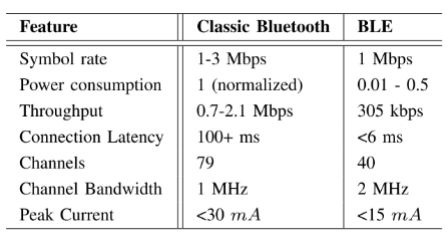
\includegraphics[width=8.5cm]{1.png}}
\caption{Classic Bluetooth And BLE Features [4]}
\label{fig}
\end{figure}\\ \\
\text{\quad} BLE devices are connectionless and periodically broadcasting their signals. These characteristics of BLE devices make them preferable to use, because they do not require device pairing to receive the BLE beacon signals. The data payload transmitted by BLE beacons is commonly called a Protocol Data Unit (PDU). Different profiles make use of PDU in different ways. For example, Apple and Google both developed their own BLE beacon protocols. \\
\text{\quad} \textit{Hardware}: As for power consumption, BLE beacons send signals periodically, and it is sufficient to evaluate its power consumption in one period, using $I_p$ and $I_i$ to represent the average current drawn during the advertisement event and the idle state respectively, the average current drawn during an advertising period can be expressed as: 
\begin{center}
$I(t_T|t_p, I_p, I_i) = \frac{t_p \cdot I_p+t_i \cdot I_i}{t_T}$
\end{center}
\text{\quad} As for BLE chipset, the standard for choosing a BLE chipset includes power consumption, flash capacity, RAM capacity, and the internal voltage regulator. Current from the radio is most significant for BLE because there is little CPU computation done in the BLE chip. Therefore, it is sufficient to analyze the current for power evaluation. The authors concludes that future researches could integrate external voltage regulator in the BLE chipset to increase battery lifetime and avoid complications.\\
\text{\quad} As for energy storage, coin-cell batteries are widely used in BLE beacon devices because of their low-profile form factor and sufficient power delivery. The disadvantage of coin-cell is that it requires frequent battery replacement due to low battery life. The use of larger alkaline batteries like AA and AAA batteries can increase the batter lifetime, but their heavy weights and large sizes are major limitations. \\ 
\text{\quad} As for energy harvest, outdoor energy harvest technology for BLE beacons includes motion and light harvesting. More complicated than outdoor energy harvest, an indoor energy harvest architecture for BLE beacon includes three parts: photovoltaic energy harvesting, power management unit, and a BLE unit. \\
\text{\quad} As for casing and installation, two major purposes for casing is look and protection. Good casing makes BLE beacons less noticeable and protects it from dust, water, or electric influences. However, one common issue is that casing needs to be cut in order to replace batteries, which makes it less protective. For installation, it is better to clear obstacles between the beacon and receiver device by setting the beacon at a height.\\
\text{\quad} \textit{Software}: As for battery monitoring, the major drawbacks of BLE beacons are the large fluctuation in RSS and a finite battery capacity, but these can be overcome through software design including battery monitoring.\\
\text{\quad} As for proximity estimation,it is essential for many BLE applications. Despite being cost-efficient, it may also cause BLE to have fluctuation in the RSS, which then affects accuracy. Fig. 2 shows estimated distance versus actual distance using RSS measurements. 
\begin{figure}[htbp]
\centerline{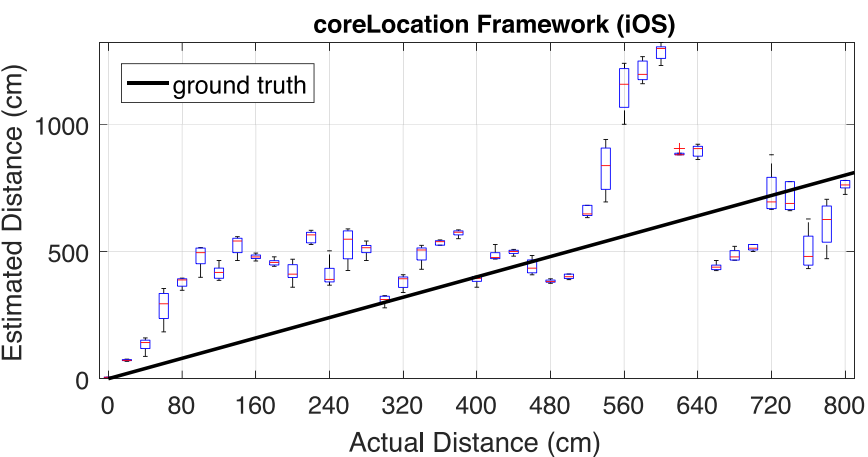
\includegraphics[width=8.5cm]{2.png}}
\caption{Eestimated Distance versus Actual Distance [4]}
\label{fig}
\end{figure} \\
\text{\quad} As for security, because of simplicity, BLE beacons can be easily attacked or abused by unwanted users. To solve this problem, the security of a BLE beacon can be protected mainly through two methods: geological validation and cloud-based token authentication.\\
\text{\quad} \textit{System Scalability}: Beacon communication is dependent on the network requests sent to the corresponding cloud servers. The number of requests is the product of total number of users and total number of beacons. Therefore, it is necessary to have a scalable server that is able to maintain successful connection rate when the number of requests and size of packets increase. 
\\
\\
\textit{L. Catarinucci et al.: An IoT-Aware Architecture for Smart Healthcare Systems}
\\
\\
\text{\quad} This paper proposes a novel, IoT-aware, smart architecture, smart hospital system (SHS), for automatic monitoring and tracking of patients, personnel, and biomedical devices within hospitals and nursing institutes. \\
\text{\quad} The smart hospital system (SHS) is consisted of following components: Ultra-high-frequency (UHF) radio frequency identification (RFID), wireless sensor network (WSN), and smart mobile, which represent three of the most promising technologies enabling the implementation of the smart healthcare system (SHS). Besides, the system also integrates 6LoWPAN and Constrained Application Protocol (CoAP), where,
\begin{itemize}
\item RFID uses electromagnetic fields to automatically identify and track tags attached to objects.
\item WSN is a network of nodes that work cooperatively to sense and control the surrounding environment.
\item 6LoWPAN is a form of WSN that sends data as packets and using IPv6 protocol.
\end{itemize}
\text{\quad} The overview of the SHS model is shown by Fig. 3, 
\begin{figure}[htbp]
\centerline{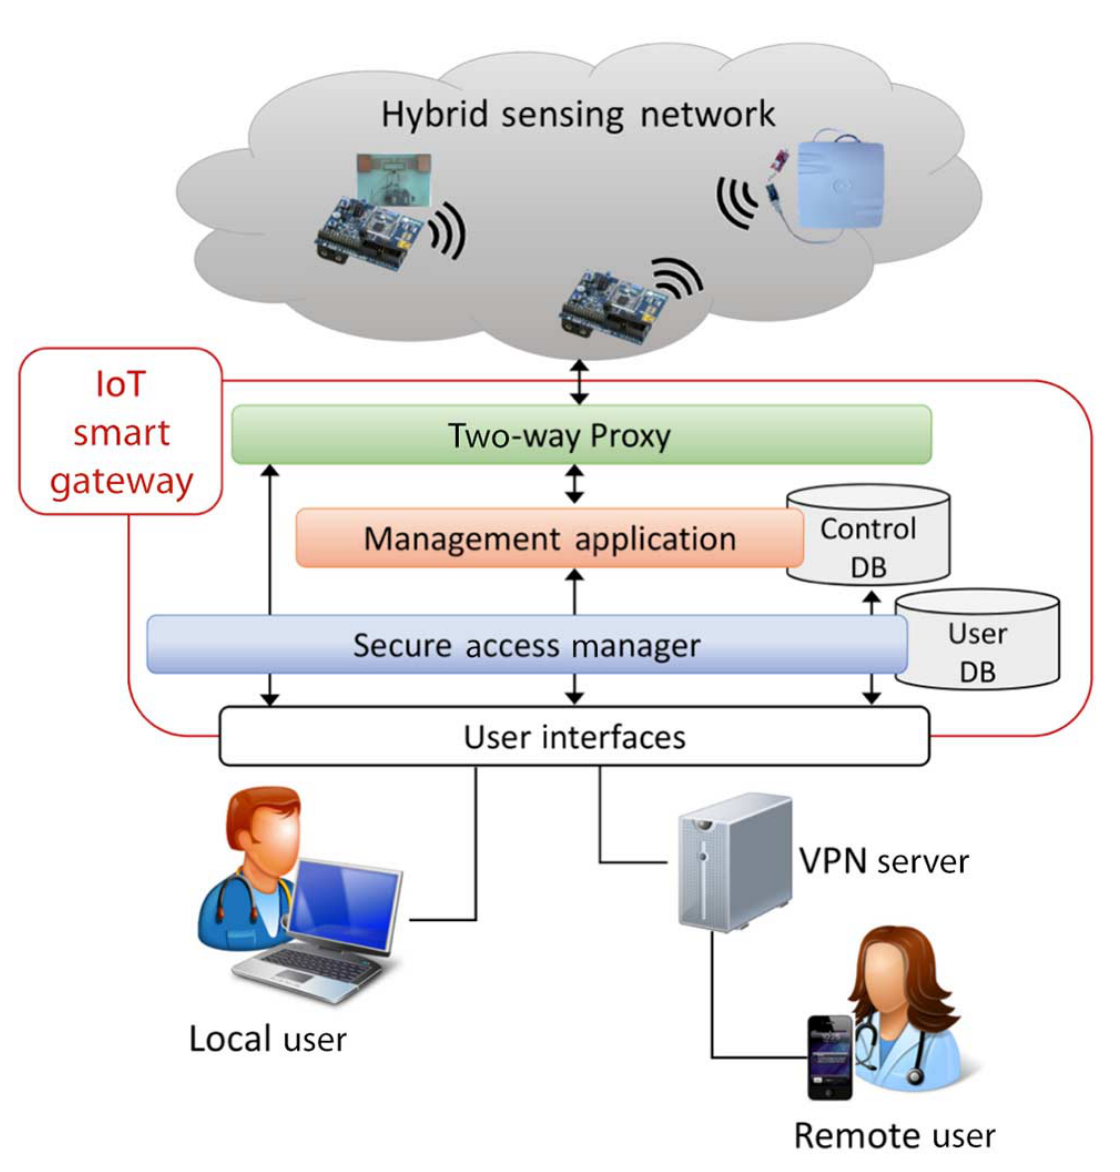
\includegraphics[width=8.5cm]{3.png}}
\caption{Overview of the SHS Architecture [1]}
\label{fig}
\end{figure}\\
\text{\quad} As for the details of the SHS architecture, it includes a Hybrid Sensing Network (HSN) consisted of an integrated
RFID-WSN 6LoWPAN network, an IoT smart gateway which represents the core of the SHS model, and user interfaces which allows authorized users to interact with the system [1].
\text{\quad} In conclusion, as long as the SHS is properly deployed and functions well, it can be a great assistance to monitor and track patients' biomedical information.
\\
\\
\textit{A. Zanella et al.: Internet of Things for Smart Cities}
\\
\\
\text{\quad} The objective of this paper is to discuss a general reference framework for the design of an urban IoT, supported by an example of large scale IoT system that has already been deployed in real world. To fulfill its objective, this paper mainly focuses on the communication between edge IoT nodes and server systems, and offers a detailed survey on IoT enabling technologies and architectures for an urban IoT.\\
\text{\quad} \textit{Services}: There are nine services discussed in this paper, the reason why these topics are of particular interest to the authors is because they improve the life quality for citizens while offer advantages to the local government by reducing its operational cost [12]. Three services, structural health, traffic management, and smart lighting, are introduced as examples.\\
\text{\quad} \textit{Architecture}: There are two main characteristics of an urban IoT infrastructure. The first characteristic is its ability to interoperate between different technologies using existing communication infrastructures. The second characteristic is the necessary accessibility of the collected data for authorities and citizens [13]. These characteristics are satisfied by appropriate combination of web service, link layers, and devices.\\
\text{\quad} \textit{Padova Smart City}: Padova Smart City is deployed at the University of Padova [14]-[15], and was originally designed to collect environmental data and monitor streetlighting by the collection of CO level, benzene level, air temperature and humidity, vibrations, and noises, while checking the operation of lighting system by monitoring light intensity at each post.
\text{\quad} In Padova Smart City, each streetlight is identified by an IoT node attached to it, which is equipped with photometer sensors, humidity sensors, and temperature sensors. There is also one benzene sensor deployed. The IoT nodes are sealed inside transparent plastic shields to prevent environmental influence and are powered by small batteries.
\text{\quad} This example is a classic representative of an urban IoT design because it involves various devices and link layer technologies. For example, IPv6 addresses are compressed through 6LoWPAN standard, and are assigned to each node to form a 6LoWPAN multihop cloud using IEEE 802.15.4 technology. A sink node is used to gather all data and interface with external nodes, which are enabled by the WAN gateway. Data are collected by the database server through communication with the HTTP-CoAP proxy server, and later can be accessed by traditional web programming.\\
\section{Problems Solved}
This section talks about the problems each paper solved, and the future researches that can be done to improve IoT enabling technologies and their applications.\\
\\
\textit{Y. Chen and T. Kunz: Performance Evaluation of IoT Protocols under a Constrained Wireless Access Network}
\\
\\
\text{\quad} In terms of software availability, implementation readiness, 
and support environments of the protocols, this paper finds that the source code of 
OpenDDS as an implementation of DDS is provided in full on 
its website and is well documented, but MQTT is not. 
Additionally, MQTT has a versatile variety of implementations 
and possesses many online resources on forums and 
communities. In contrast, the open source implementation of 
CoAP is less readily available and poorly supported or 
commentated [3]. \\
\text{\quad} As for protocol performance, DDS has the largest bandwidth consumption compared with other three protocols, MQTT has the largest experienced latency while the other three protocols have rather acceptable latencies. Overall, CoAP can be the best candidate if the computation and internet resources are limited. \\
\text{\quad} However, the research on only four protocols is not enough as IoT applications are becoming more and more popular, therefore, future researches on other M2M protocols, such as AMQP and JMS are recommended by the authors to be performed.
\\
\\
\textit{K. E. Jeon et al.: BLE Beacons for Internet of Things Applications Survey, Challenges, and Opportunities}
\\
\\
\text{\quad} The challenges for BLE beacons mainly lie on three aspects: protocol, hardware, and software.\\
\text{\quad} \textit{BLE Protocols}: Two major BLE protocols are iBeacon and Eddystone, which are incompatible with each other. Thus, it is important for a mobile device such as a smart phone to support both protocols, so that it can connect to the most of Bluetooth devices. Upon the compatibility challenge, BLE protocols are also facing the signal interfering challenge, because there are usually many-to-many Bluetooth connections within a region. To account for this challenge, RSS-comparison [16] is designed such that only the beacon with the strongest RSS will be connected. The RSS-comparison technology is not suitable under every condition, and more decent algorithm for selecting connection should be developed. Moreover, there are different interaction interfaces that may cause development challenges if beacons do not use the same interfacing technology. \\
\text{\quad} \textit{Hardware}: The major challenge for BLE hardware is the energy harvesting technology. Although energy harvesting has been studied for Wireless Sensor Networks (WSN), it is not sufficient for BLE beacons, because WSNs are mostly outdoor systems while BLE beacons are used both indoor and outdoor. Also, the electrical characteristics of BLE beacons are different from wireless sensors. Therefore, researchers can focus on developing hardware specifications for BLE beacons to suit different scenarios. \\
\text{\quad} \textit{Software}: The main software challenges for BLE beacons include battery monitoring, distance estimation, system scalability, and security.\\
\text{\quad} As for battery monitoring, the challenge is that BLE beacons cannot update battery information frequently with low user traffic nearby, and errors might exist in the retrieved battery level because each beacon may have different battery information packet offset. Therefore, the battery information should be considered to get accurate battery data. \\
\text{\quad} As for distance estimation, the identification of beacons by measuring RSS in a dense environment is challenging because there is an interference among close beacons. Future researches can study the algorithm to improve the accuracy of RSS measurement. \\
\text{\quad} As for system scalability, many network requests are generated by multiple devices at the same time, which require proper management. A possible approach to improve the server performance is by reducing the number of requests needed.\\
\text{\quad} As for security, the geological validation and cloud-based token authentication are more like precautionary systems rather than security systems, for they prevent beacon abuses, but cannot detect or react to potential attacks. The research on security issues in BLE beacon infrastructure is still at its starting up stage and there is little research done. So the authors launch an urgent call for a more scalable attack detection method with less computational load, as well as a security protocol to fully control the beacon network. \\
\\
\textit{L. Catarinucci et al.: An IoT-Aware Architecture for Smart Healthcare Systems}
\\
\\
\text{\quad} This paper gives a novel, IoT-aware, SHS architecture for
automatic monitoring and tracking of patients, personnel, and
biomedical devices within hospitals and nursing institutes [1]. The IoT system of the SHS is complex but robust, because CoAP, 6LoWPAN, and REST paradigms are integrated into the model, allowing interaction with UHF RFID Gen2, WSN, and smart mobile
technologies. \\
\text{\quad} However, there still exist some possibilities for the SHS to be improved, for example, cloud computing can be integrated into the system to handle larger amount of patients' data. Additionally, a security system can be designed to improve the protection of patients' privacy.
\\
\\
\textit{A. Zanella et al.: Internet of Things for Smart Cities}
\\
\\
\text{\quad} This paper not only introduces an entire IoT system for Smart Cities application, but also surveys on the difficulties that slow down the popularization of Smart Cities application. \\ 
\text{\quad} \textit{Political Obstacles}: One major problem of Smart Cities is the administration power attribution to different stakeholders. This may be solved by institutionalizing the decision-making process into one department to prevent the attribution of decision-making power to different stakeholders [17]. \\
\text{\quad} \textit{Technical Issues}: There still exists noninteroperability issue of current heterogeneous technologies, which should be solved by building an unified urban-scaled ICT platform based on IoT vision [18]-[19].\\
\text{\quad} \textit{Financial Problems}: The market still lacks a clear business model. To account for this, investors can first try Smart Cities services that have clear and direct return on investment such as smart parking, and then aid the deployment of other added-value services [20].
\\
\section{Strategies of Each Paper}
This section discusses the strategies of each paper, which gives readers insight into the methodology of IoT research.\\
\\
\textit{Y. Chen and T. Kunz: Performance Evaluation of IoT Protocols under a Constrained Wireless Access Network}
\\
\\
\text{\quad} This paper selects three quantitative metrics, bandwidth consumption, experienced latency, and experienced packet loss, to indicate protocol performance. By varying system latency, system packet loss, and network bandwidth cap independently through network emulation tools NetEM and TBF, the quantitative metrics are measured with several independent variable settings. To enhance the reliability of the study, Y. Chen and T. Kunz made all three trials for each independent variable setting are set to run 
for $10$ minutes and $3$ repetitions with the final reported result being the average of them. 
\\
\\
\textit{K. E. Jeon et al.: BLE Beacons for Internet of Things Applications Survey, Challenges, and Opportunities}
\\
\\
\text{\quad} This paper uses three strategies to study the BLE beacon technology: survey on existing works, comparison between different approaches, and small-scale experiments.\\
\text{\quad} For example, the authors conducted an experiment on CR2450 battery with a nominal voltage of 3 V (2-3.6V working range) to show that CyPhy Media iOS application can provide approximate battery information. In Fig. 4, in contrast to the actual battery voltage and percentage provided by the mobile application, it can be concluded that the behavior of CR2450 is consistent with its theoretical characteristics [21].
\begin{figure}[htbp]
\centerline{
\includegraphics[width=8.5cm]{4.png}}
\caption{Mobile Application Reported Battery Level versus Actual Voltage of CR2450 battery [4]}
\label{fig}
\end{figure}
\\
\textit{L. Catarinucci et al.: An IoT-Aware Architecture for Smart Healthcare Systems}
\\
\\
\text{\quad} This paper introduces how an IoT system can be an integration of different hardware and software components. The authors breaks the SHS model into a Hybrid Sensing Network (HSN) consisted of an integrated
RFID-WSN 6LoWPAN network, an IoT smart gateway which represents the core of the SHS model, and user interfaces which allows authorized users to interact with the system [1], such that each module is designed and improved in parallel.
\\
\\
\textit{A. Zanella et al.: Internet of Things for Smart Cities}
\\
\\
\text{\quad} This paper has three strategies to present the IoT system for Smart Cities applications: literature review, comparison between different methods, and field experiment.\\
\text{\quad} For example, for the data collection of field experiment of Padova Smart City, temperature, humidity, light, and benzene readings over a period of 7 days are demonstrated in this paper. Red dots represent raw data, and the lines stand for the average value within one hour. From Fig. 5(a), it can be observed that the light reaches its peaks at daytime and reaches minimum at night. The light intensity value is noisy at night because of the influence of car lights. The Benzene level in Fig. 5(b) is lower at night because of lower traffic congestion.
\begin{figure}[htbp]
\centerline{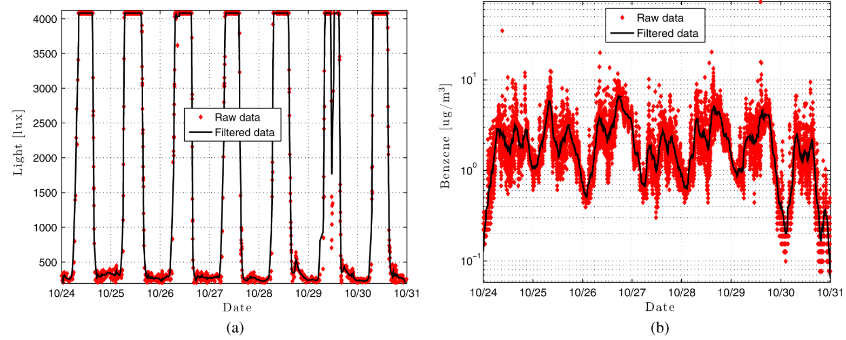
\includegraphics[width=8.5cm]{5.png}}
\caption{Data Collected in the Padova Smart City: (a) Light and (b) Benzen [2]}
\label{fig}
\end{figure}
\section{Conclusion}
During the past decades, the IoT technology has exhibited its great potential to improve the living standards of mankind, to reduce government operational cost, as well as to elevate the urban service. Therefore, recognizing the fast-growing development of IoT enabling technologies is becoming an increasingly important topic. This paper surveys on some representative IoT enabling technologies such as protocols and devices, and digs into real-world IoT applications, especially two practical IoT integrated systems, Smart Hospital Systems (SHS) and Smart Cities. As a conclusion, Y. Chen and T. Kunz worked out a quantitative approach to evaluate IoT protocols, according to three metrics, bandwidth consumption, experienced latency, and experienced packet loss. Based on their experiment, CoAP is considered as a protocol with the most promising performance in resource-limited IoT applications. As for K. E. Jeon and his team, they studied on BLE beacons (although this technology is still at its infant level), and found the great potential strengths that might make future researches on BLE beacons worthwhile, including the interoperability between devices, sustainability, security protocol, and etc. Furthermore, L. Catarinucci and his colleagues proposed a SHS model that is able to monitor the biomedical data of patients and send off emergency alerts. This SHS is realized mainly by three technologies, UHF, RFID, and WSN. It demonstrates the advantage of an IoT-based system that can provide low power remote health condition monitoring and real-time emergency checking. Lastly, the blueprint of Smart Cities IoT integrated solution deployed in Padova was comprehensively investigated by A. Zanella and her colleagues. Their work shows the Smart Cities can be a representitive example for a complete IoT system including web service, link layer technologies, sensors, and other devices. However, although IoT enabling technologies and IoT applications are now becoming more and more mature, there still exist some technical, financial, and even political obstacles that prevent the popularization of IoT systems, therefore, future studies on how to improve the performance, enhance the security, and lower down the cost of IoT technology are still necessary for researchers.

\section*{Acknowledgment}

This work is supported by Prof. Volodymyr Kindratenko's IoT \& Cognitive Computing course project. The authors would like to thank Prof. V. Kindratenko for his assistance and suggestions. They would also thank Prof. Deming Chen and other teaching staff for providing course materials.

\begin{thebibliography}{00}
\bibitem{b1} L. Catarinucci et al, ``An IoT-Aware Architecture for Smart
Healthcare Systems", IEEE Internet of Things Journal, vol. 2, pp. 515-526, 27 Mar. 2015.
\bibitem{b2} A. Zanella et al, ``Internet of Things for Smart Cities", IEEE Internet of Things Journal, vol. 1, pp. 22-32, 14 Feb. 2014.
\bibitem{b3} Y. Chen and T. Kunz, ``Performance Evaluation of IoT Protocols under a Constrained Wireless Access Network", 2016 International Conference on Selected Topics in Mobile and Wireless Networking (MoWNeT), pp. 1-7, Apr. 2016.
\bibitem{b4} K. E. Jeon, ``BLE Beacons for Internet of Things Applications: Survey, Challenges, and Opportunities,'' IEEE Internet of Things Journal, vol. 5, pp. 811-828, 1 Jan. 2018.
\bibitem{b5} MQTT Protocol Specification, http://mqtt.org. 
\bibitem{b6} CoAP Protocol Specification, http://coap.technology.
\bibitem{b7} DDS Protocol Specification, http://www.omg.org/spec/DDS. 
\bibitem{b8} XMPP Protocol Specification, http://xmpp.org.
\bibitem{b9} R. Faragher and R. Harle, “Location fingerprinting with Bluetooth low energy beacons”, IEEE J. Sel. Areas Commun., vol. 33, no. 11, pp. 2418–2428, Nov. 2015.
\bibitem{b10} A. Cunningham, “Explaining Continuity: The Tech Tying iOS 8 and OS X Yosemite Together", [Online], Available: https:// arstechnica.com/gadgets/2014/07/explaining-continuity-the-tech-tyingios-8-and-os-x-yosemite-together/, Jul. 2014.
\bibitem{b11} Y. Kashimoto et al., “Sensing activities and locations of senior citizens toward automatic daycare report gener-ation”, in Proc. IEEE 31st Int. Conf. Adv. Inf. Netw. Appl. (AINA), Taipei, Taiwan, pp. 174–181, Mar. 2017.
\bibitem{b12} M. Dohler et al., “Smart Cities: An Action Plan”, Proc. Barcelona Smart Cities Congress, Barcelona, Spain, pp. 1–6., Dec. 2011.
\bibitem{b13} C. E. A. Mulligan and M. Olsson, “Architectural implications of smart city business models: An evolutionary perspective”, IEEE Commun. Mag., vol. 51, no. 6, pp. 80–85, Jun. 2013.
\bibitem{b14} A. P. Castellani et al., “Web services for the Internet of Things through CoAP and EXI”, Proc. IEEE Int. Conf. Commun. (ICC 2001), Kyoto, Japan, 2011.
\bibitem{b15} P. Casari et al., “The WIreless SEnsor networks for city-WideAmbient Intelligence (WISE-WAI) project”, MDPIJ. Sensors, vol. 9, no. 6, pp. 4056–4082, [Online], Available: http://www.mdpi.com/1424-8220/9/6/4056, Jun. 2009.
\bibitem{b16} I. Howitt, “Mutual interference between independent Bluetooth piconets”, IEEE Trans. Veh. Technol., vol. 52, no. 3, pp. 708–718, May 2003.
\bibitem{b17} I. Vilajosana et al., “Bootstrapping smart cities through a self-sustainable model based on big data flows”, IEEE Commun. Mag., vol. 51, no. 6, pp. 128–134, Jun. 2013.
\bibitem{b18}J. M. Hernández-Muñoz et al., “Smart Cities at the forefront of the future Internet”, The Future Internet, Lect. Notes Comput. Sci., vol. 6656, pp. 447–462, 2011.
\bibitem{b19} C. E. A. Mulligan and M. Olsson, “Architectural implications of smart city
business models: An evolutionary perspective”, IEEE Commun. Mag.,
vol. 51, no. 6, pp. 80–85, Jun. 2013.
\bibitem{b20} N. Walravens and P. Ballon, “Platform business models for smart cities: From control and value to governance and public value”, IEEE Commun. Mag., vol. 51, no. 6, pp. 72–79, Jun. 2013.
\bibitem{b21} Energizer CR2450, [Online], Available: http://data.energizer.com/pdfs\\/cr2450.pdf.

\end{thebibliography}

\end{document}
